\documentclass[12pt]{article}
\usepackage[utf8]{inputenc}

\usepackage{graphicx}       

      
\title{\textbf{Tarea de Medición de Tiempo en C++}}
\author{Lipa Quispe Alex Dannis}
\date{\today}

\begin{document}

\maketitle


\section*{\textbf{Descripción del Código}}
La principal estructura del código se basa en abrir un archivo `.txt` para luego almacenar sus datos en un arreglo.

Una vez guardados estos valores, el código encargado de ordenar el arreglo es **QuickSort**, lo que permite buscar los números de manera más rápida y eficiente.

Posteriormente, el programa solicita al usuario la cantidad de números que desea buscar. Una vez ingresados estos valores, el programa identifica en qué posición se encuentra cada número y el tiempo que demoró en encontrarlo.  
Finalmente, compara los tiempos de búsqueda, mostrando en pantalla los números con los tiempos máximos y mínimos.

\section*{\textbf{Código del Programa}}

\newpage
\begin{figure}[t]
    \centering
    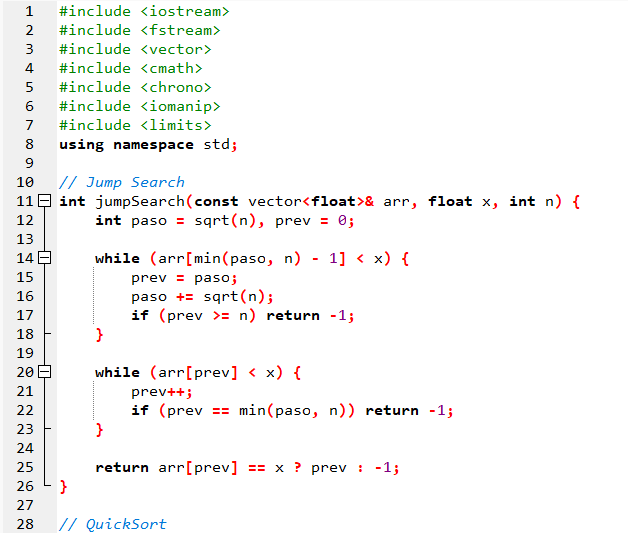
\includegraphics[width=0.7\textwidth]{imagen1.png}
    \caption{Función que se encarga de buscar los valores deseados.}
    \label{fig:codigo-busqueda}
\end{figure}

\begin{figure}[t]
    \centering
    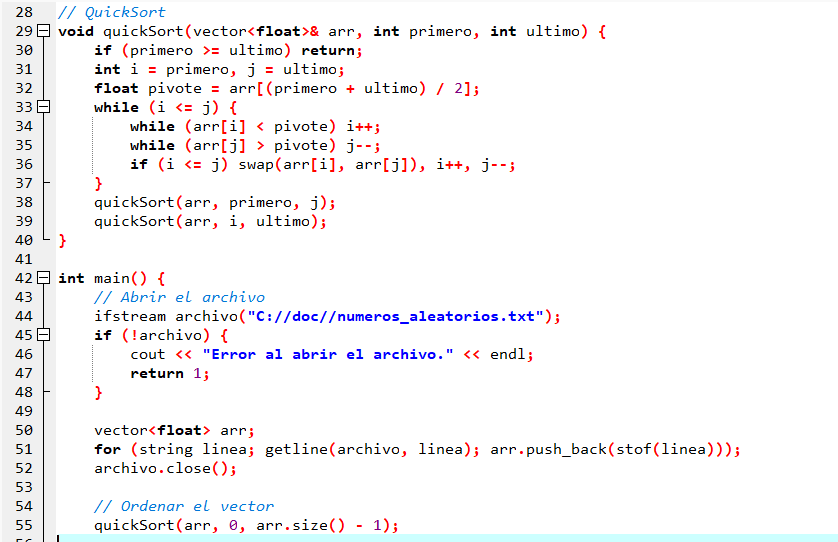
\includegraphics[width=0.7\textwidth]{imagen2.png}
    \caption{Función que ordena los datos del archivo utilizando QuickSort.}
    \label{fig:codigo-quicksort}
\end{figure}

\begin{figure}[t]
    \centering
    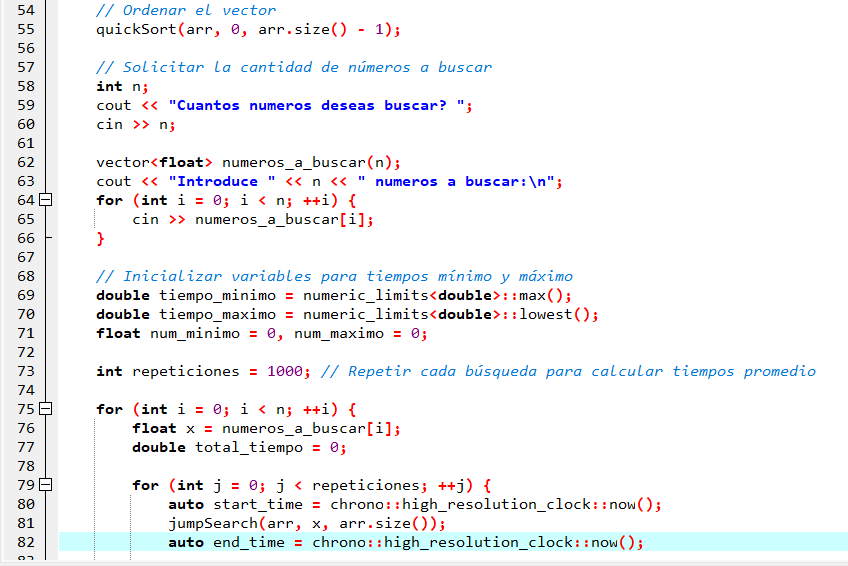
\includegraphics[width=0.7\textwidth]{imagen3.png}
    \caption{Estructura principal del programa llamando las funciones necesarias.}
    \label{fig:estructura-principal}
\end{figure}
\begin{figure}
    \centering
    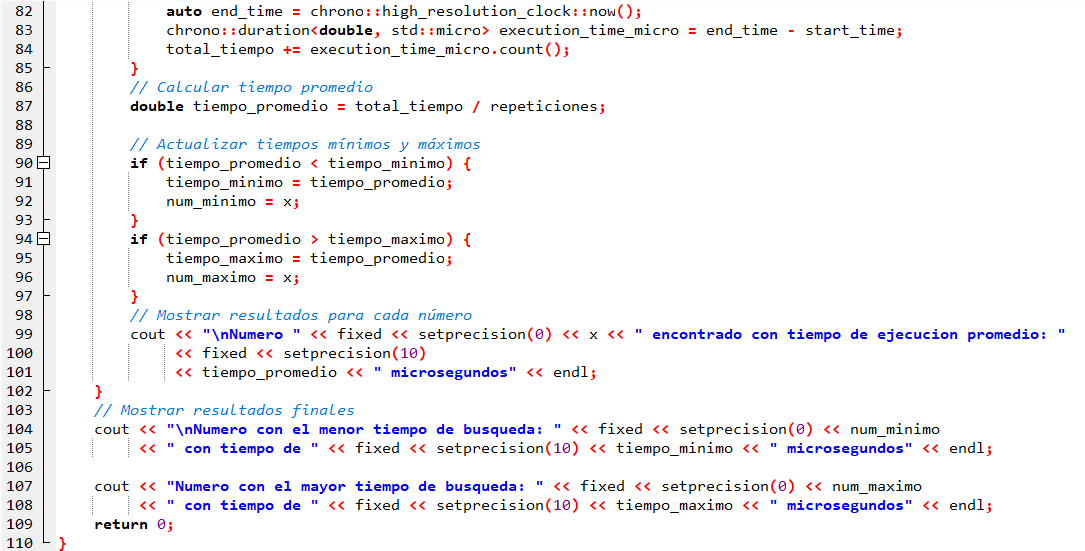
\includegraphics[width=0.7\linewidth]{imagen4.png}
    \caption{Parte final del código donde calcula y verifica el mayor y menor tiempo en hacer la búsqueda}
    \label{fig:enter-label}
\end{figure} 
\clearpage 
Una vez de haber escrito de manera ordenado y estructurada el código se procede a compilar el código:
\begin{figure}
    \centering
    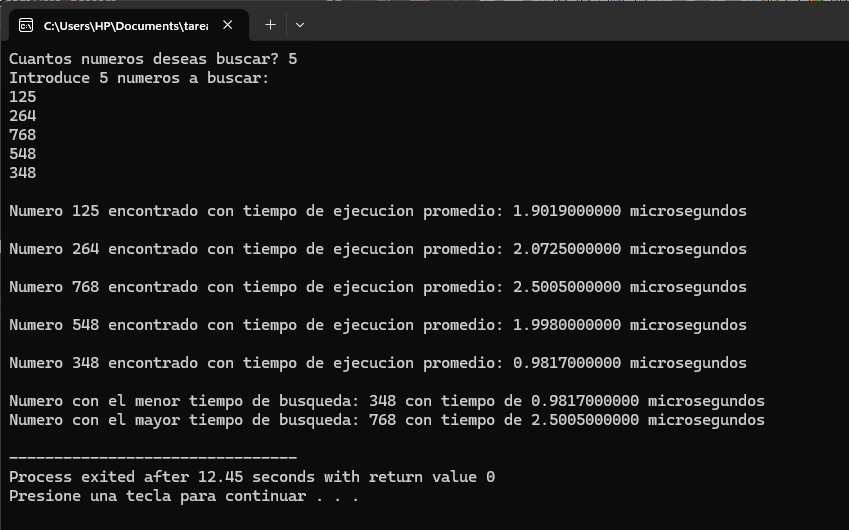
\includegraphics[width=0.7\linewidth]{imagen5.png}
    \caption{El progrma se compilo correctamente}
    \label{fig:enter-label}
\end{figure}
\end{document}